\documentclass[11pt]{beamer}

% Presento style file
%\usepackage{config/presento}

% custom command and packages
% custom packages
\usepackage{textpos}
\setlength{\TPHorizModule}{1cm}
\setlength{\TPVertModule}{1cm}

\newcommand\crule[1][black]{\textcolor{#1}{\rule{2cm}{2cm}}}



\usepackage[spanish]{babel}
\selectlanguage{spanish} 
\usepackage[utf8]{inputenc}
\usepackage{default}
\usetheme{CambridgeUS}
%\usecolortheme{dolphin}
\usecolortheme{seahorse}
\usepackage{graphicx}
\usepackage{float} % supuestamente sirve para las tablas, con [H] se ponen en donde uno quiere
\restylefloat{table} % supuestamente sirve para las tablas, con [H] se ponen en donde uno quiere
\usepackage{amsmath}
% limits underneath
\DeclareMathOperator*{\argmax}{arg\,max} % Jan Hlavacek
\DeclareMathOperator*{\argmin}{arg\,min} % Jan Hlavacek
\usepackage{subfig}    %para hacer figuras multiples
%\usepackage{hyperref}
\usepackage{cancel}



% Information
\title{Machine Learning en Astronom\'{\i}a}
\subtitle{Segundo seminario de Doctorado}
\author{Bruno S\'anchez \& \\
Mariano Dom\'{\i}guez}
\titlegraphic{
\includegraphics[scale=0.8]{./images/vitraux_h90.png}}
\institute{IATE - FaMAFyC} %\\
%
\includegraphics[scale=0.8]{./images/vitraux_h90.png}}
\date{\today}

\begin{document}

% Title page
\begin{frame}[plain]
\maketitle
\end{frame}

% sections in the presentation
% \begin{frame}{Resumen}
%  \begin{fullpageitemize}
%   \item \largetext{Motivaciones}
%   \item \largetext{Las diferencias de im\'agenes}
%   \item \largetext{Pipelines con Corral}
%   \item \largetext{Simulaciones de im\'agenes}
%   \item \largetext{Datos reales}
%   \item \largetext{Machine Learning}
%  \end{fullpageitemize}
% \end{frame}

\begin{frame}
\frametitle{Contenidos}
\tableofcontents%[sectionstyle=show/hide, sectionstyle=show/shaded]
\end{frame}


\section{Motivaciones}

\begin{frame}{Variabilidad el cielo}
    \begin{figure}
        \centering
        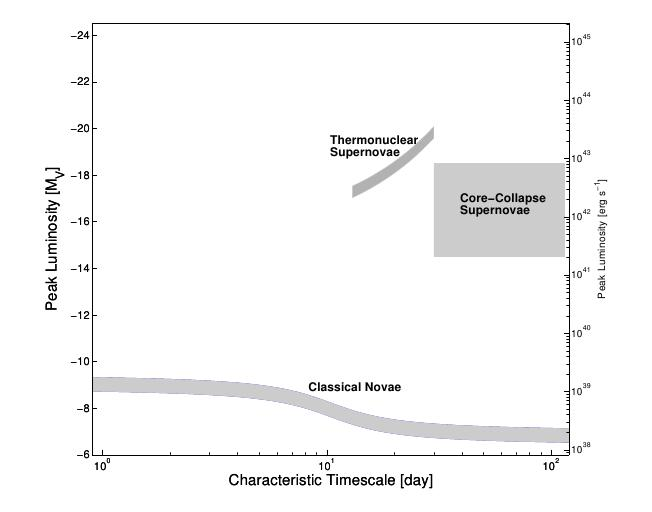
\includegraphics[width=0.7\textwidth]{./images/imgs_seminario1/diag1.jpeg}
        \caption{Diagrama de variabilidad (Kasliwal et al 2012)}
        \label{fig:diag_vacio}
    \end{figure}
\end{frame}

\begin{frame}{Variabilidad en el cielo}
    \begin{figure}
        \centering
        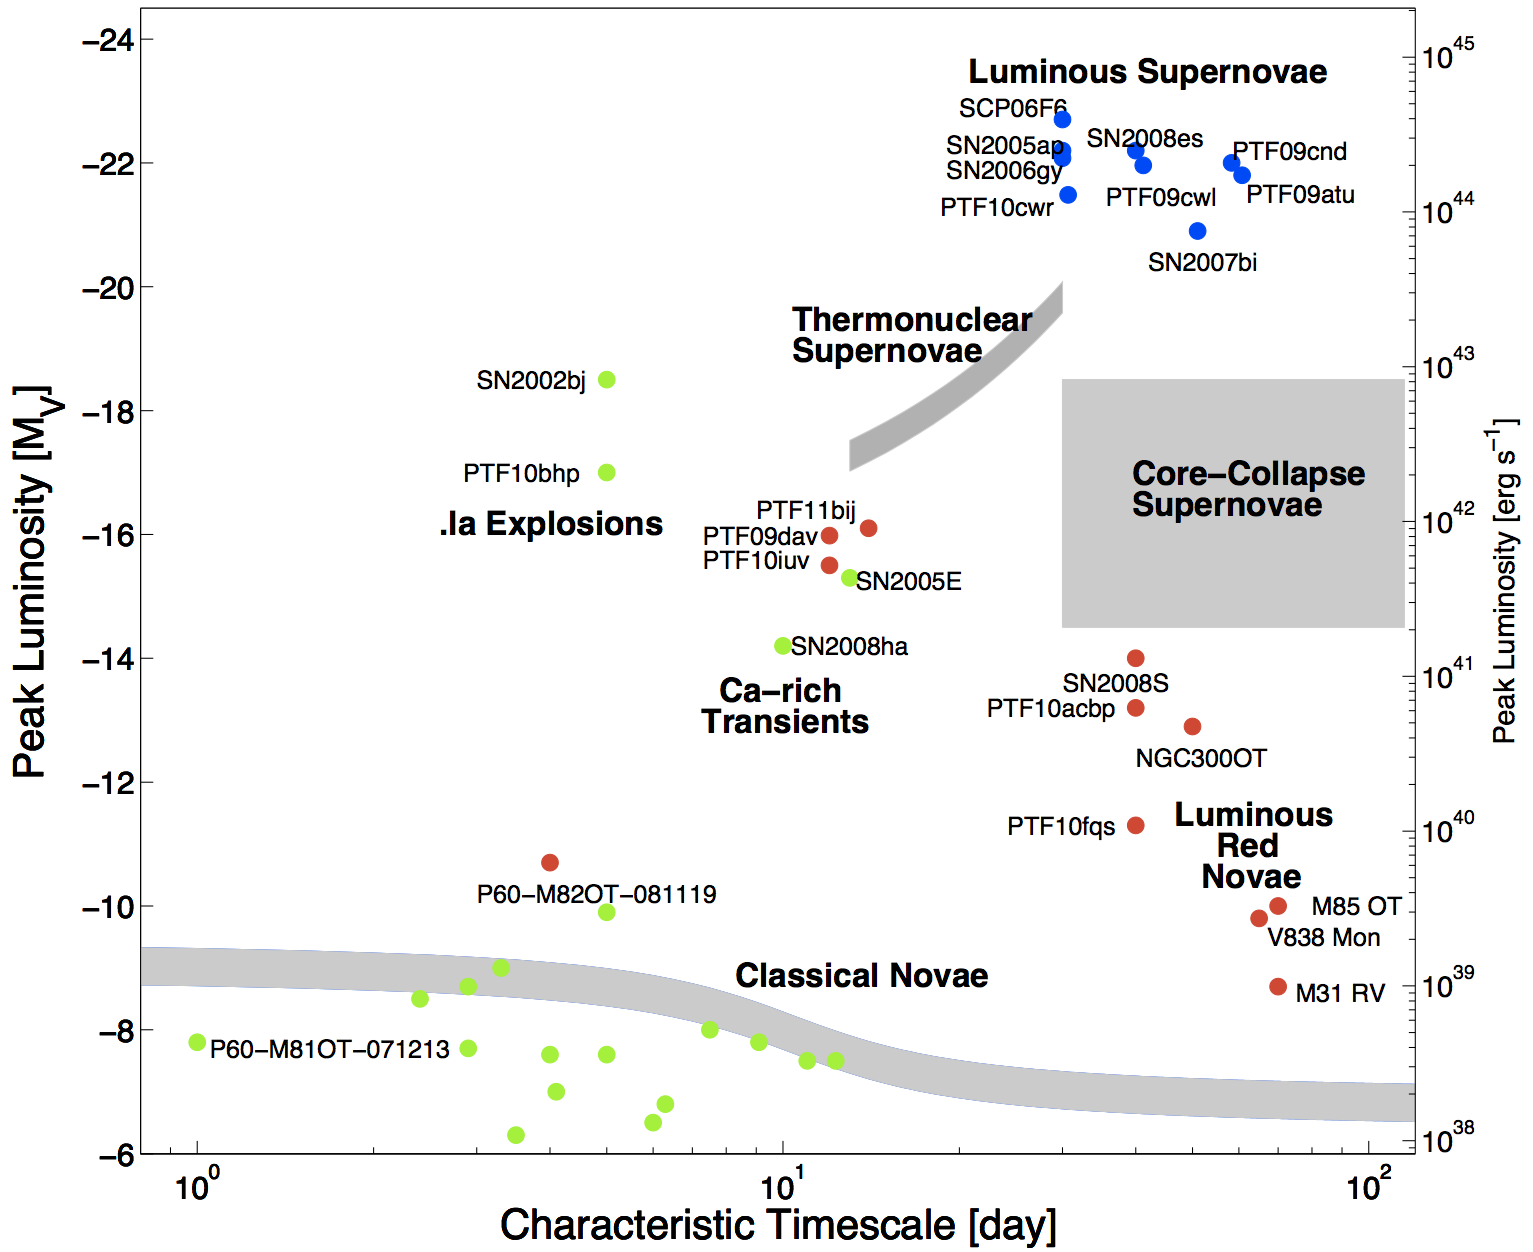
\includegraphics[width=0.65\textwidth]{./images/imgs_seminario1/taumv.png}
        \caption{Diagrama de variabilidad (Kasliwal et al 2012)}
        \label{fig:diag_lleno}
    \end{figure}
\end{frame}

\begin{frame}{Large Synoptic Survey Telescope}
    \begin{figure}
        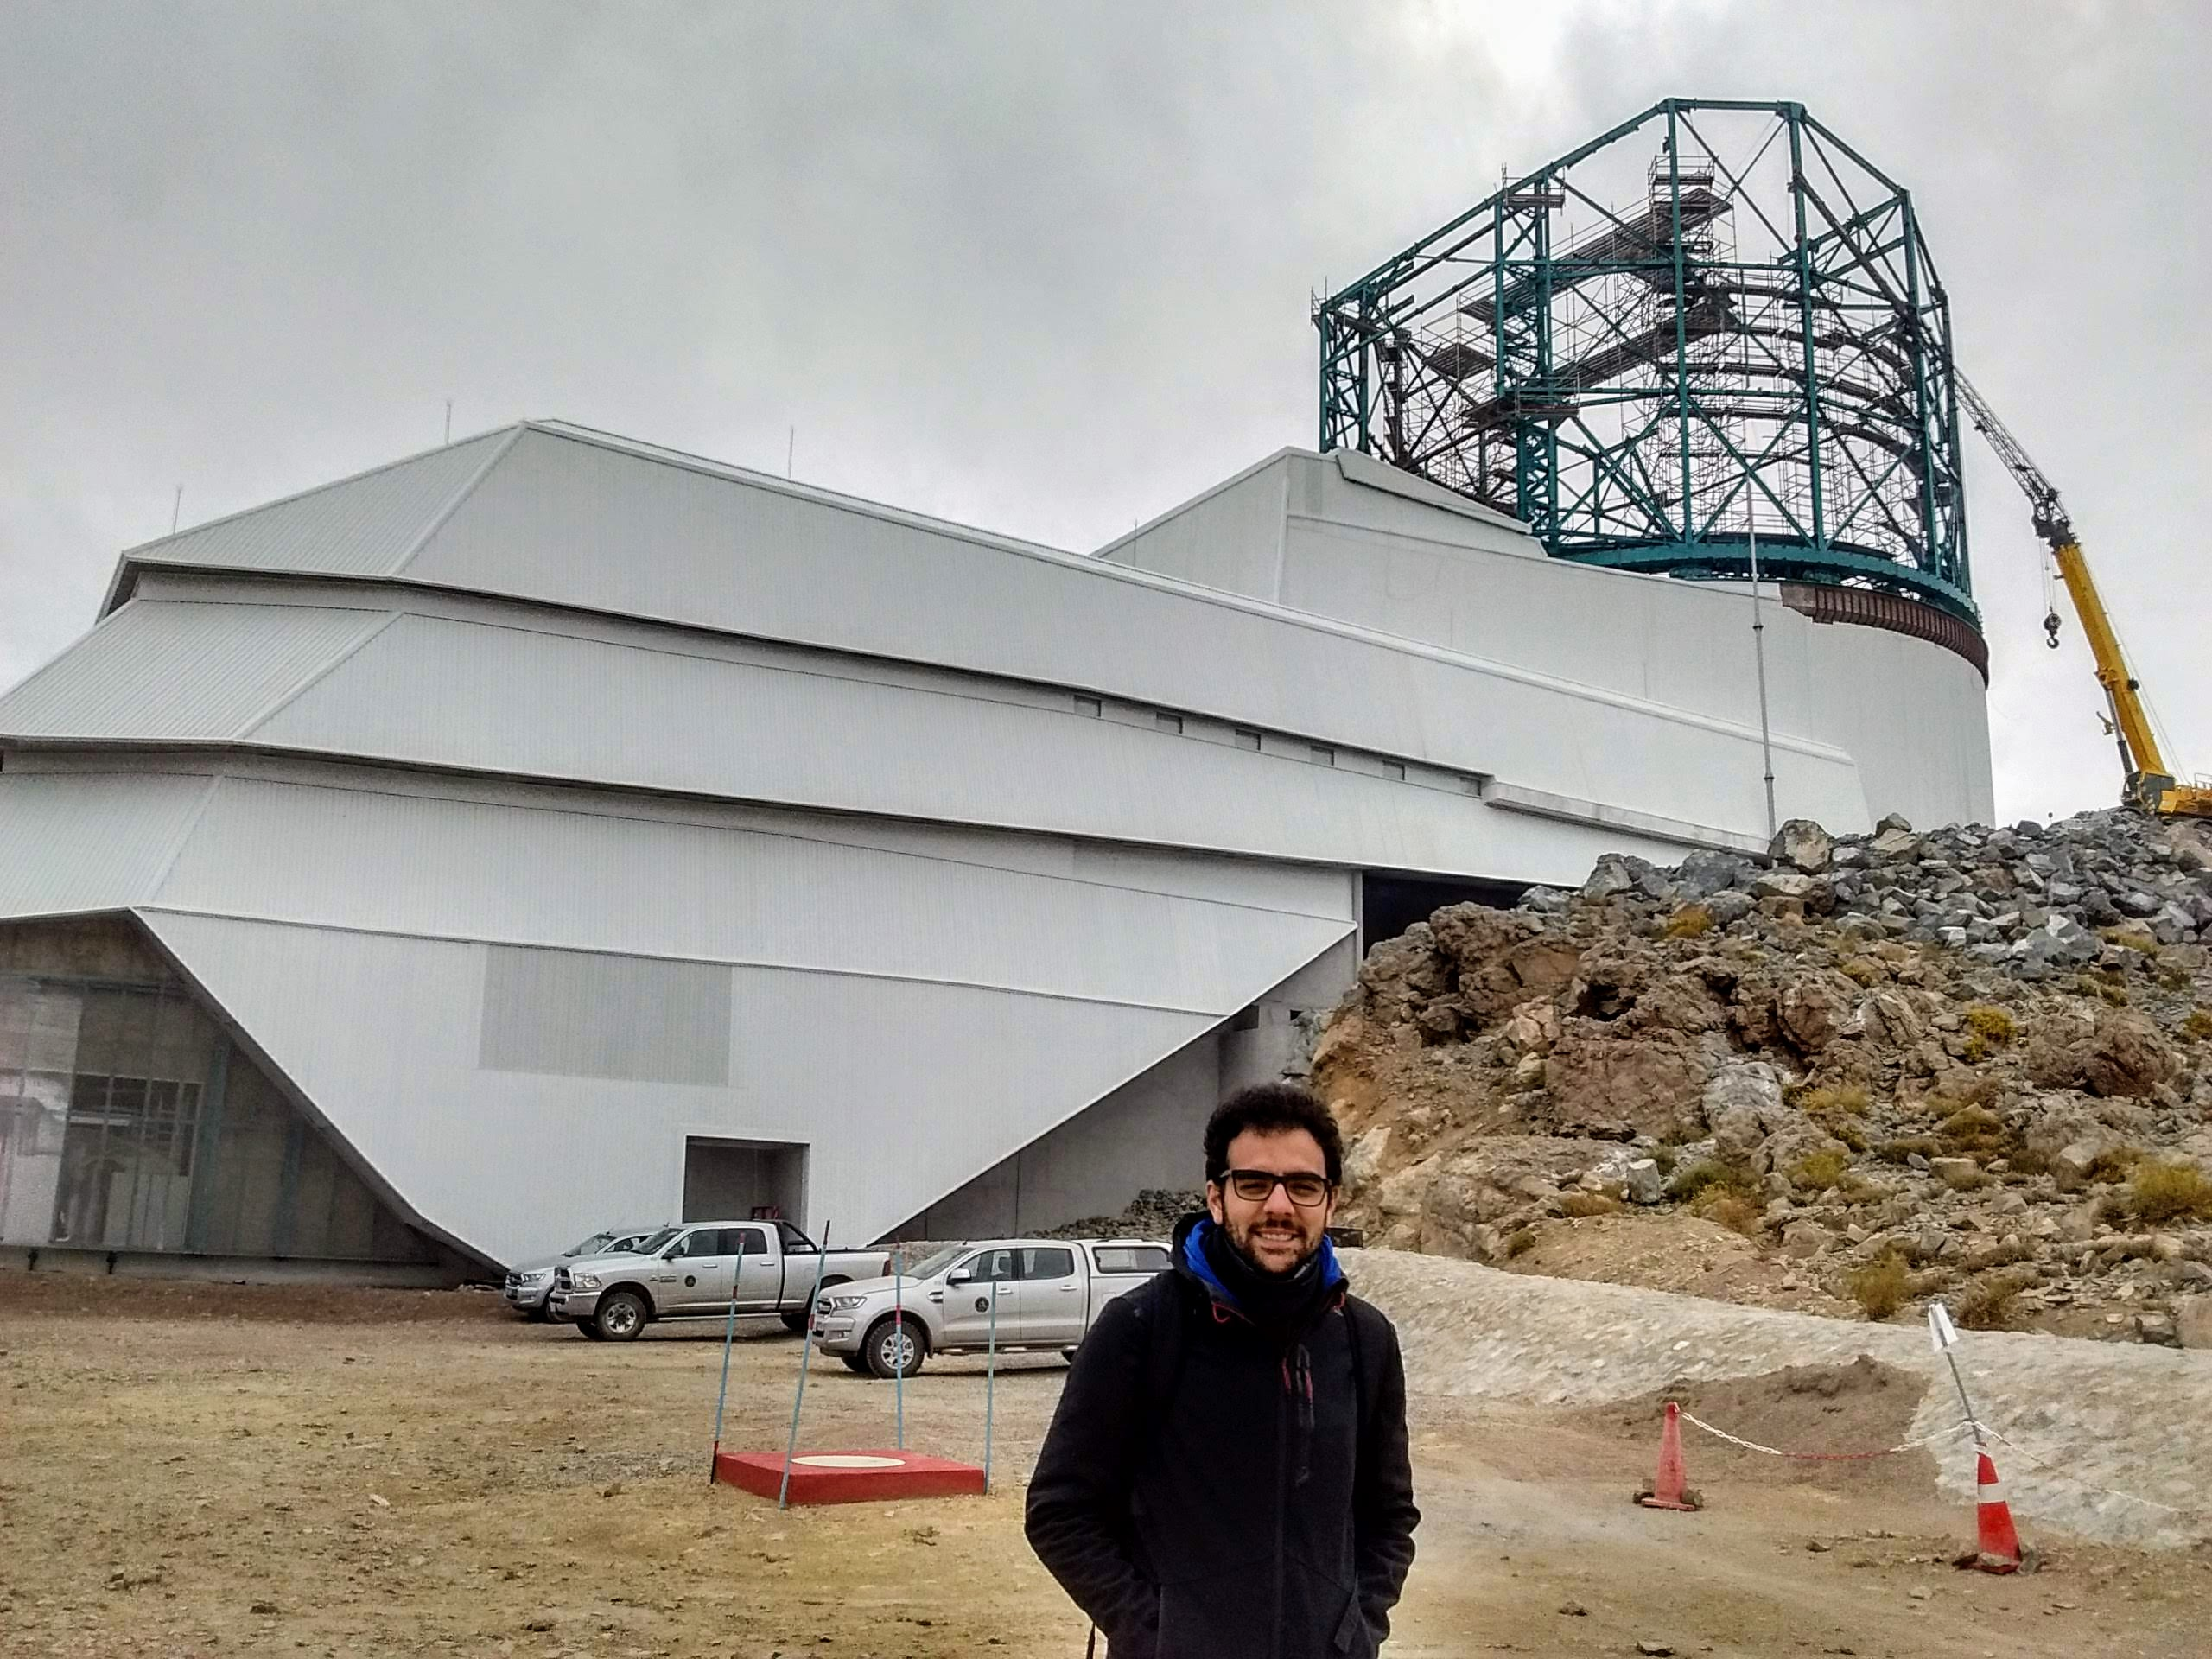
\includegraphics[width=0.45\textwidth]{./images/yo+LSST.jpg}
        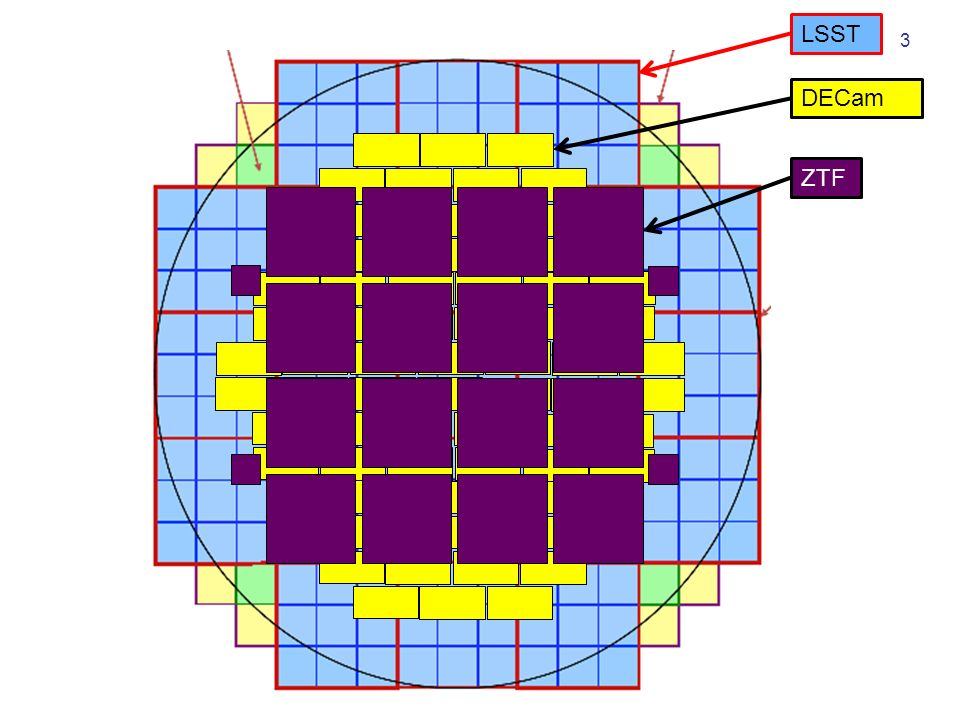
\includegraphics[width=0.45\textwidth]{./images/imgs_seminario1/LSST+DECam+ZTF.jpg}
        \caption{LSST construcci\'on y c\'amara \textit{footprint}}
        \label{fig:camaras}
    \end{figure}
\end{frame}



\begin{frame}{Las diferencias de im\'agenes (DIA)}
Pros \& Cons
   \begin{exampleblock}{Localizado}
   Se pueden encontrar eventos dentro de objetos extendidos
   \end{exampleblock}
   \pause
   \begin{exampleblock}{Sensible}
   Se pueden detectar objetos d\'ebiles
   \end{exampleblock}
   \pause
   \begin{alertblock}{Artefactos de la sustracci\'on}
   La operaci\'on tiene resultados inestables
   \end{alertblock}
   
\end{frame}

\begin{frame}{Distintos tipos de operaciones DIA}
    Primeros intentos: \cite{phillips_registering_1995}
    
    Hoy existen diferentes t\'ecnicas de sustracci\'on de im\'agenes:
    \begin{itemize}
        \item Alard \& Lupton \cite{alard_method_1998}
        \item Bramich \cite{bramich_new_2008}
        \item Zackay, Ofek and Gal-Yam \cite{zackay_proper_2016}
    \end{itemize}
\end{frame}

\begin{frame}{Conexi\'on con el ML}
    A pesar de ser diferentes las t\'ecnicas, 
    todas poseen defectos:
    \begin{figure}
        \centering
        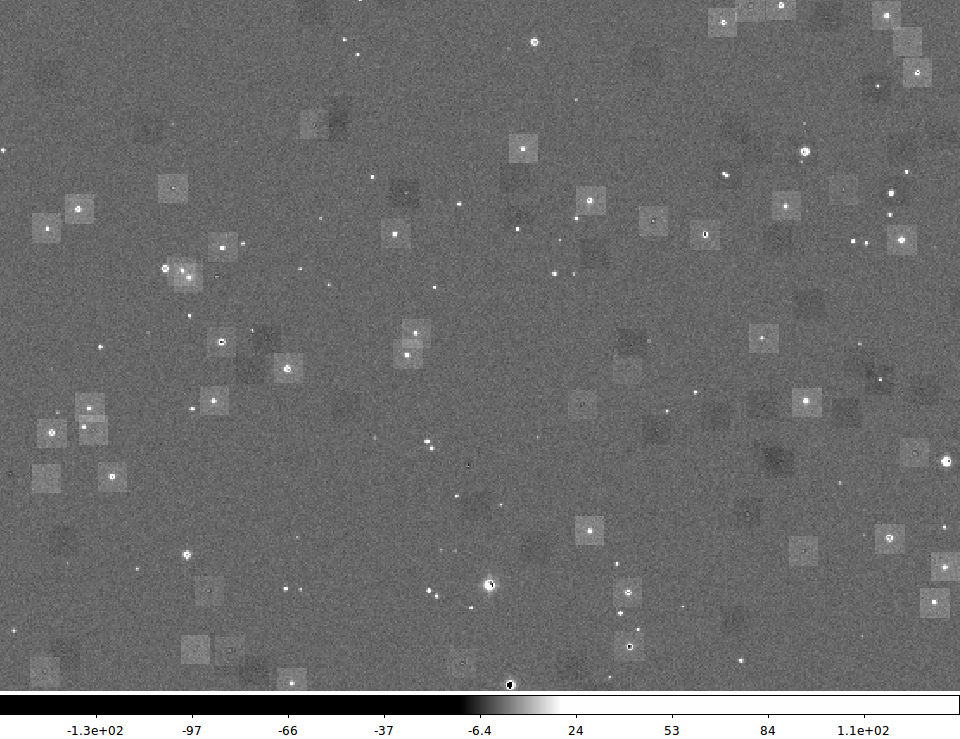
\includegraphics[width=0.33\textwidth]{images/diff.png}
        %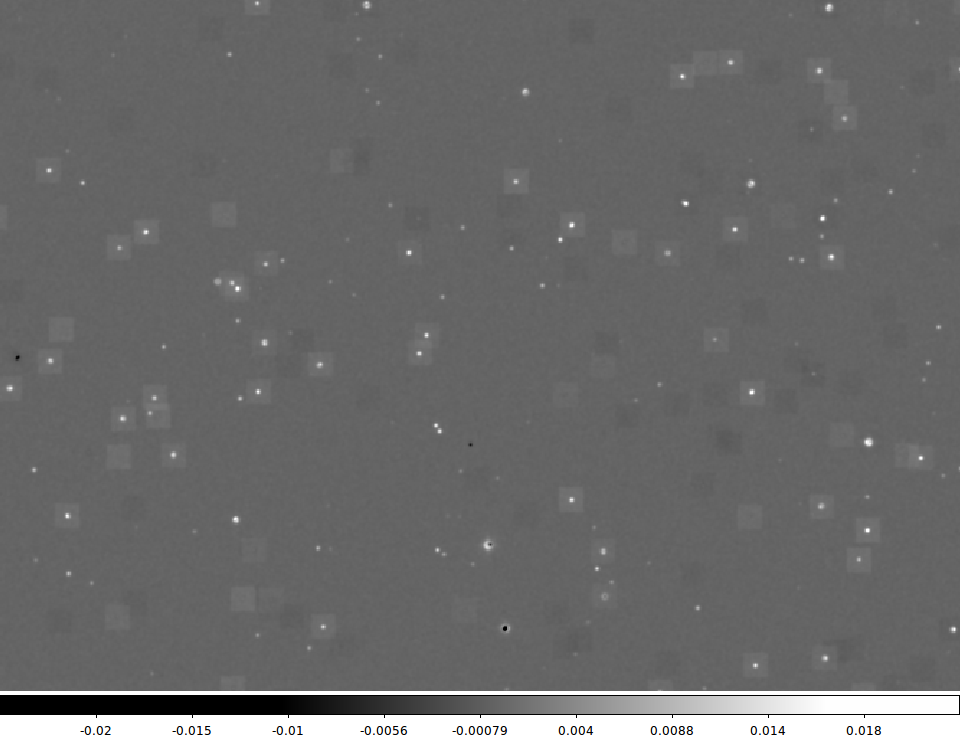
\includegraphics[width=0.23\textwidth]{images/s_diff.png}
        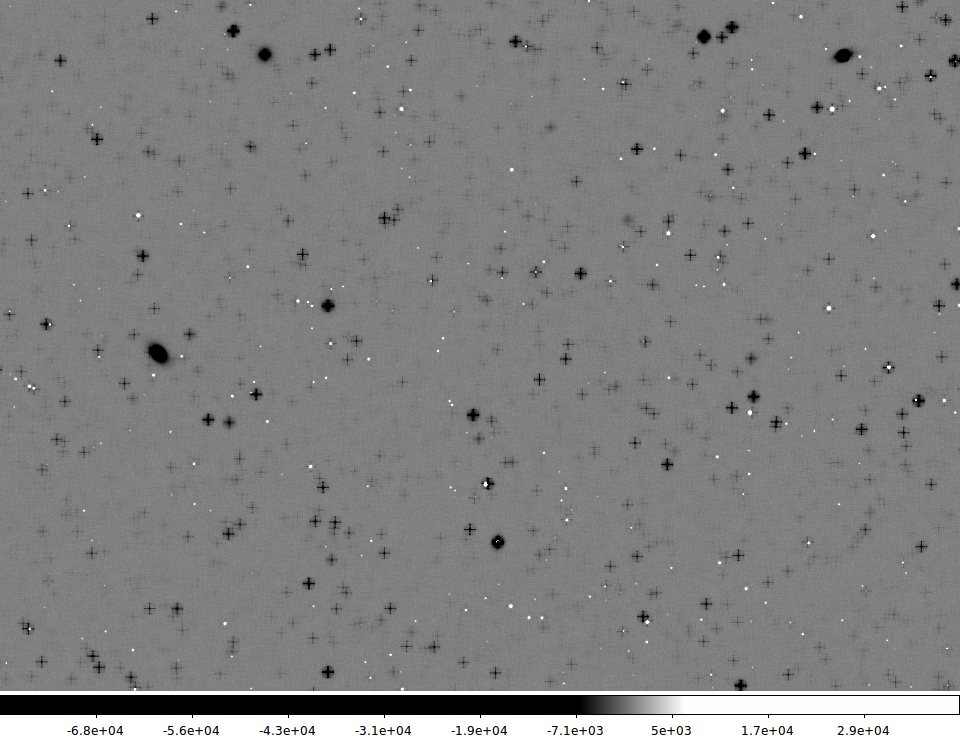
\includegraphics[width=0.33\textwidth]{images/diff_ois.png}
        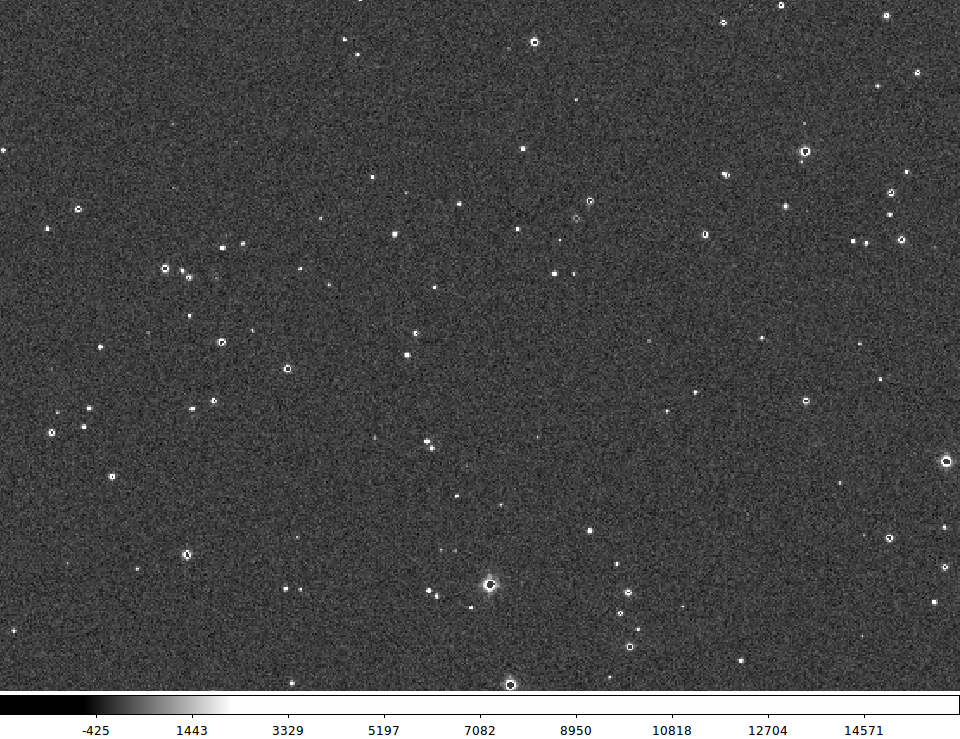
\includegraphics[width=0.33\textwidth]{images/diff_hot.png}
        \caption{Izq. Zackay, centro Bramich, der. A\&Lupton.}
        \label{fig:restas}
    \end{figure}
    
    Es importante entonces poder discriminar las detecciones reales de las esp\'ureas,
    y el ML nos ahorra tiempo y es reproducible.
    \end{frame}

%-----------------------------------------------------------------------------
\begin{frame}[fragile]{Astronom\'{\i}a $=>$ Big Data}
\small
\begin{table}[]
\begin{tabular}{ccc}
Sky Survey \footcite{garofalo2016astrophysics}  & Volumen & Velocidad       \\ \hline
% \begin{tabular}[c]{@{}c@{}}SDSS \rule{0pt}{3ex}\\ \textit{Sloan Digital Sky Survey}\end{tabular}                                              & 50 TB  & 200 GB per day \\
% GAIA \rule{0pt}{3ex} & 100 TB & 40 GB per day  \\
% \begin{tabular}[c]{@{}c@{}}Pan-STARRS \rule{0pt}{3ex}\\ \textit{Panoramic Survey Telescope}\\ \textit{and Rapid Response System}\end{tabular} & 5 PB   & 5 TB per day   \\
% \begin{tabular}[c]{@{}c@{}}LSST \rule{0pt}{3ex}\\ \textit{Large Synoptic Survey Telescope}\end{tabular}                              & 60 PB  & 10 TB per day  \\
% \begin{tabular}[c]{@{}c@{}}SKA \rule{0pt}{3ex}\\ \textit{Square Kilometer Array}\end{tabular}                                        & 3 ZB   & 150 TB per day
\end{tabular}
\end{table}
\normalsize
\end{frame}

%-------------------------------------------------------------------------------
\begin{frame}[fragile]{Aplicaciones en Astronom\'{\i}a}
	\vbox to .9\vsize{
	\small 
	\begin{itemize}
	    \item Determinaci\'on de \textit{Redshift} Fotom\'etricos (1706.02467 y 1806.06607)
	    \item Clasificaci\'on morfol\'ogica de galaxias (1809.08377)
	    \item B\'usqueda de transitorios en tiempo real (1708.08947 y 1710.01422)
        \item Clasificaci\'on de curvas de luz (1709.06257)
        \item Modelado de PSF (\textit{Fast Point Spread Function}) (1801.07615)
        \item Detecci\'on de Supernovas (1808.03626)
        \item Medici\'on de Lentes Gravitacionales D\'ebiles y fuertes (1807.02120, 1703.02642 y 1808. 00011)
        \item Simulaci\'on de cat\'alogos (1709.09665)
        \item Detecci\'on de \textit{Cosmological Diffuse Radio Sources} (1809.03315)
        \item Cosmolog\'{\i}a para estructuras de gran escala (1808.04728)
        \item An\'alisis de im\'agenes de rayos gamma (1810.00591)
        \item Detecci\'on de ondas gravitacionales (1711.03121)
	\end{itemize}
	\normalsize
	}
\end{frame}	
%-------------------------------------------------------------------------------
\section{Machine Learning}
\subsection{Introducci\'on}
\begin{frame}{Algunas definiciones del ML}


    A. Samuel (1956):
    \begin{quote}
        Un campo de estudio que le da la habilidad a una computadora de aprender sin ser explicitamente programada
    \end{quote}
    T. Mitchel (1998):
    \begin{quote}
        Estudio de algoritmos que mejoran la perfomance $P$ en alguna tarea $T$ con la experiencia $E$
    \end{quote}
\end{frame}
%-------------------------------------------------------------------------------
\begin{frame}{Un breve esquema}
    %Como forma de trabajo se cambia totalmente la mec\'anica:
    \begin{figure}
        \centering
        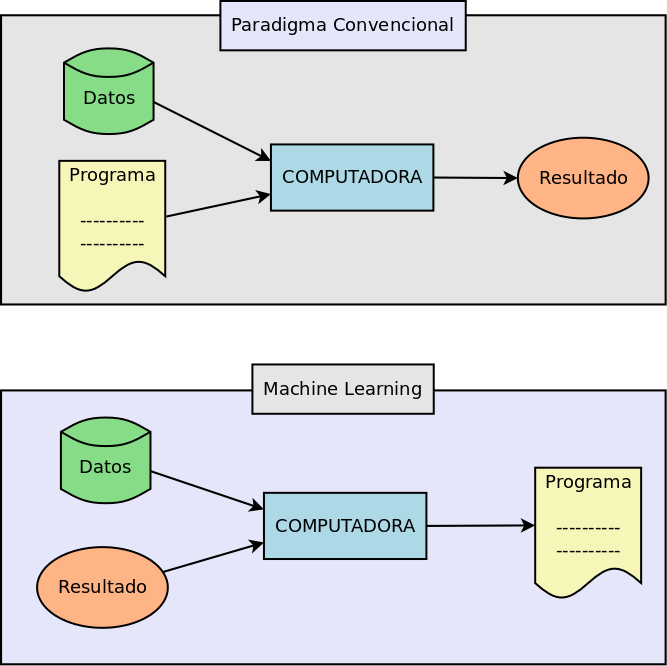
\includegraphics[width=0.6\textwidth]{images/ML_vs_programming.png}
        %\caption{}
        \label{fig:ML_vs_conventional}
    \end{figure}
\end{frame}
%-------------------------------------------------------------------------------
\begin{frame}{Hitos del ML}
\begin{itemize}
    \item[1936] Alan Turing y su "M\'aquina Universal"
    \item[1951] Primer red neuronal
    \item[1952] Arthur Samuel, y su m\'aquina que juega Damas
    \item[1959] MADALINE: una de las primeras redes neuronales de uso comercial. Reduce el ruido de llamadas telef\'onicas.
    \item[1967] Se inventa \textit{k-Nearest Neighbors}
    \item[1969] Se publica un trabajo con fuertes conclusiones sobre las limitaciones de las Redes Neuronales artificiales.
    \item[70-80] \textit{AI's winter} o Invierno de IA
\end{itemize}
\end{frame}
\begin{frame}{Hitos del ML}
\begin{itemize}
    \item[1986] Algoritmo de entrenamiento de redes: \textit{Backpropagation}
    \item[1995] Se inventa \textit{Random Forest y Support Vector Machines}
    \item[1997] Kasparov pierde su famosa partida ante una computadora IBM
    \item[2006] Resurgimiento de las redes, a trav\'es del \textit{Deep Learning}
    \item[2011] Watson gana en el concurso \textit{Jeopardy!}
    \item[2014] El test de Turing es superado por primera vez
    \item[2016] Por primera vez una computadora gana una partida de GO ante un campe\'on humano
    \item[2018] \textit{Auto-ML}
\end{itemize}
\end{frame}
%-------------------------------------------------------------------------------
\begin{frame}{Formalizaci\'on}
    
\end{frame}

%-------------------------------------------------------------------------------
\begin{frame}{Tipos de ML}
Hay distintos tipos de Machine Learning:
\begin{columns}
\begin{column}{0.3\textwidth}
    \begin{itemize}[<+->]
        \item Aprendizaje supervisado
        \item Aprendizaje \textbf{NO}-supervisado
        \item Reinforcement learning (basado en recompensas)
        %\item Aprendizaje semi-supervisado
    \end{itemize}
\end{column}
\begin{column}{0.7\textwidth}
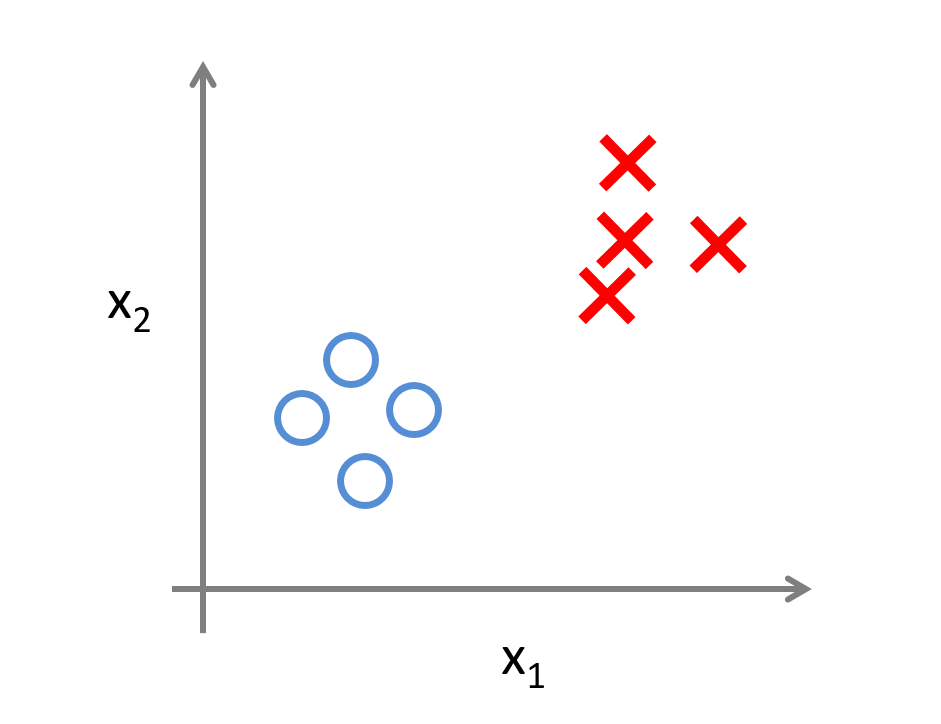
\includegraphics[width=0.5\textwidth]{images/supervised.png}
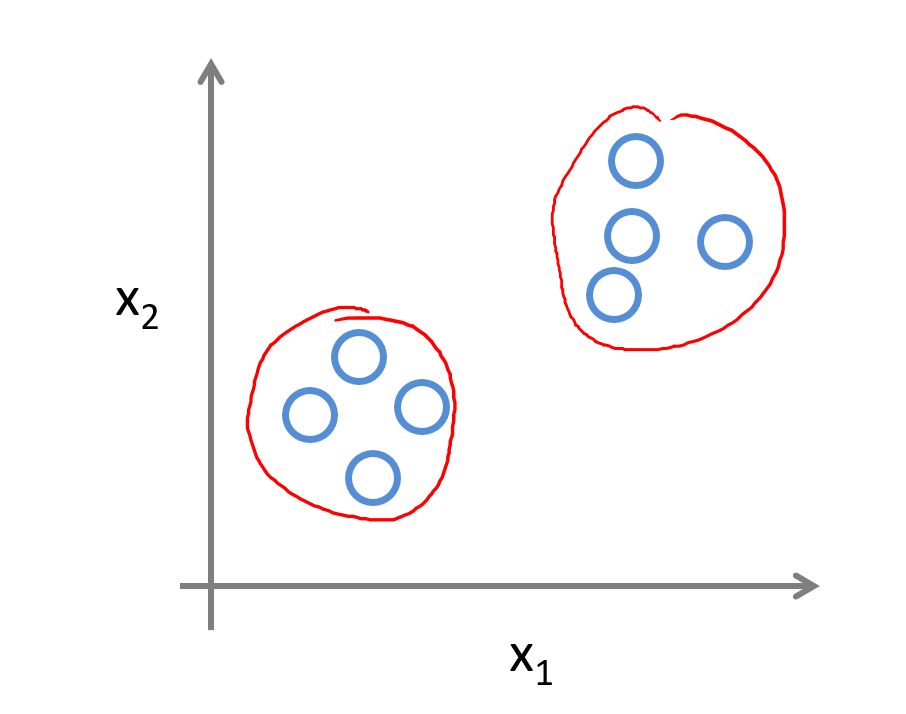
\includegraphics[width=0.5\textwidth]{images/unsupervised.png}
\end{column}
\end{columns}
\end{frame}
%-------------------------------------------------------------------------------
\begin{frame}{Para fijar ideas...}
    Las aplicaciones m\'as comunes del ML engloban
    \begin{itemize}
        \item Clasificaci\'on
        \item Regresi\'on
        \item Clustering
        \item Reconocimiento de patrones en im\'agenes
        \item Mucho m\'as
    \end{itemize}
\end{frame}
%-------------------------------------------------------------------------------
\begin{frame}{Formalizando}
\begin{itemize}
    \item Un conjunto de N datos de entrada llamados instancias $\{\vec{f}_i\}$ (\'o $\{\vec{x}_i\}$).
    \begin{itemize}
        \item Estos son vectores de dimensi\'on $d$, y cada una se denomina \textit{feature} o variables descriptora.
        \item Pueden ser n\'umeros reales, categor\'ias, o variables \textit{bool}.
    \end{itemize}
    \item Adem\'as es posible tener la clase objetivo o $y_i$: el resultado a \textit{aprender}.
    \item Normalmente dividimos el conjunto de datos en \textit{conjunto de entrenamiento} y otro \textit{conjunto de validaci\'on}.
\end{itemize}
\end{frame}
%-------------------------------------------------------------------------------
\begin{frame}{Ciclo de ML}
\begin{figure}
    \centering
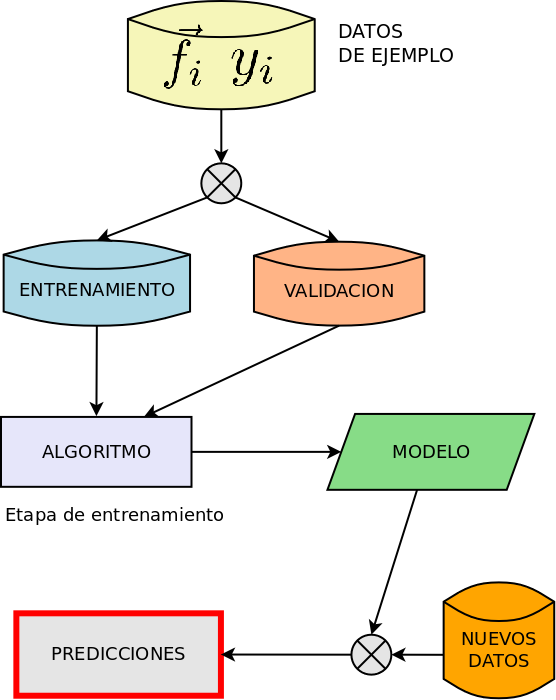
\includegraphics[width=0.45\textwidth]{images/ml_cycle.png}
    \label{fig:ml_cycle}
\end{figure}
\end{frame}
%-------------------------------------------------------------------------------
\subsection{Los Algoritmos de ML}
\begin{frame}{Algoritmos de Machine Learning}
    Un algoritmo se compone de tres elementos:
    \begin{itemize}%[<+->]
        \item Representaci\'on\only<2>
            {: \textit{el tipo de modelo que utilizaremos para predecir}}
        \item Evaluaci\'on\only<3>
            {: \textit{la funci\'on que maximizaremos para que nuestro modelo pueda aprender}}
        \item Optimizaci\'on\only<4>
            {: \textit{la estrategia de b\'usqueda de los par\'ametros que maximizan la funci\'on de evaluaci\'on}}
    \end{itemize}
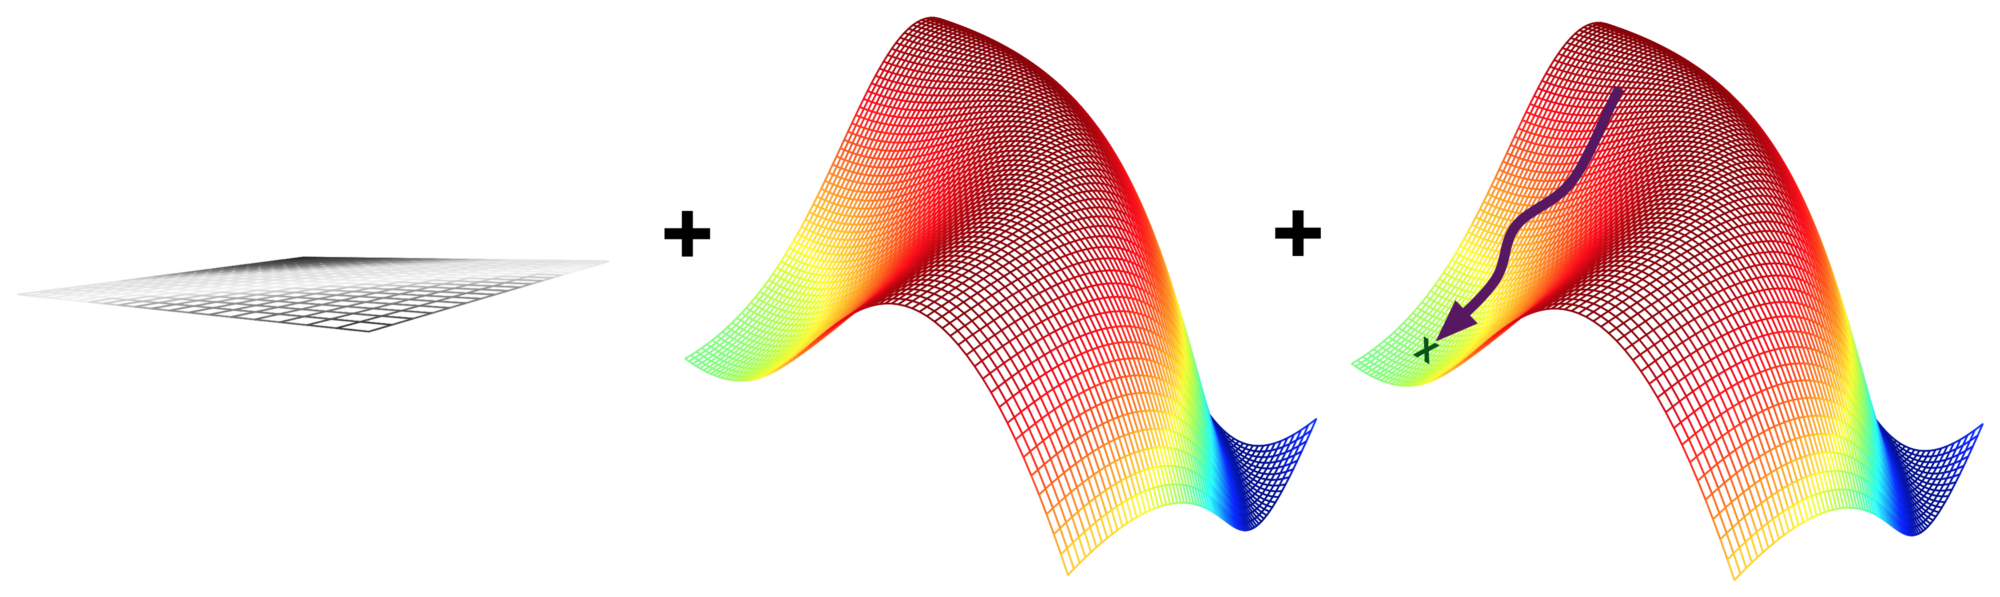
\includegraphics[width=0.9\textwidth]{images/representation+evaluation+optimization.png}
\end{frame}
%-------------------------------------------------------------------------------
\subsection{Algoritmos populares de ML}
\begin{frame}{Regresi\'on}
    
    \begin{block}{Cuadrados m\'{\i}nimos}
    Regresi\'on puede pensarse como el ajuste de funciones que ya conocemos.
    \end{block}
    
    \begin{itemize}
        \item La representaci\'on: $$y_i = a x_i + b$$
        \item La evaluaci\'on: $$\chi^2 = \sum_i(y_i - a x_i -b)^2$$
        \item La optimizaci\'on: $$\frac{\partial \chi^2}{\partial a,b} = 0$$
   \end{itemize}
\end{frame}
%-------------------------------------------------------------------------------
\begin{frame}{Ejemplos de representaci\'oon}
  Uno de los m\'as simples: \textit{K-Nearest Neighbors}
  \begin{figure}
  \centering
  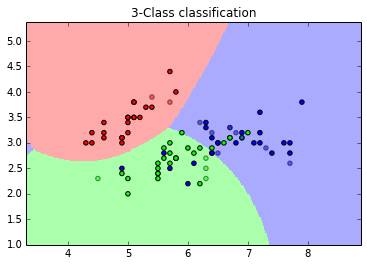
\includegraphics[width=0.7\textwidth]{images/knearest_example.png}
  \label{fig:my_label}
  \end{figure}
\end{frame}
%-------------------------------------------------------------------------------
\begin{frame}{\textit{Support Vector Machines}}
\begin{columns}[T]
    \begin{column}{0.40\textwidth}
    \begin{figure}
        \centering
        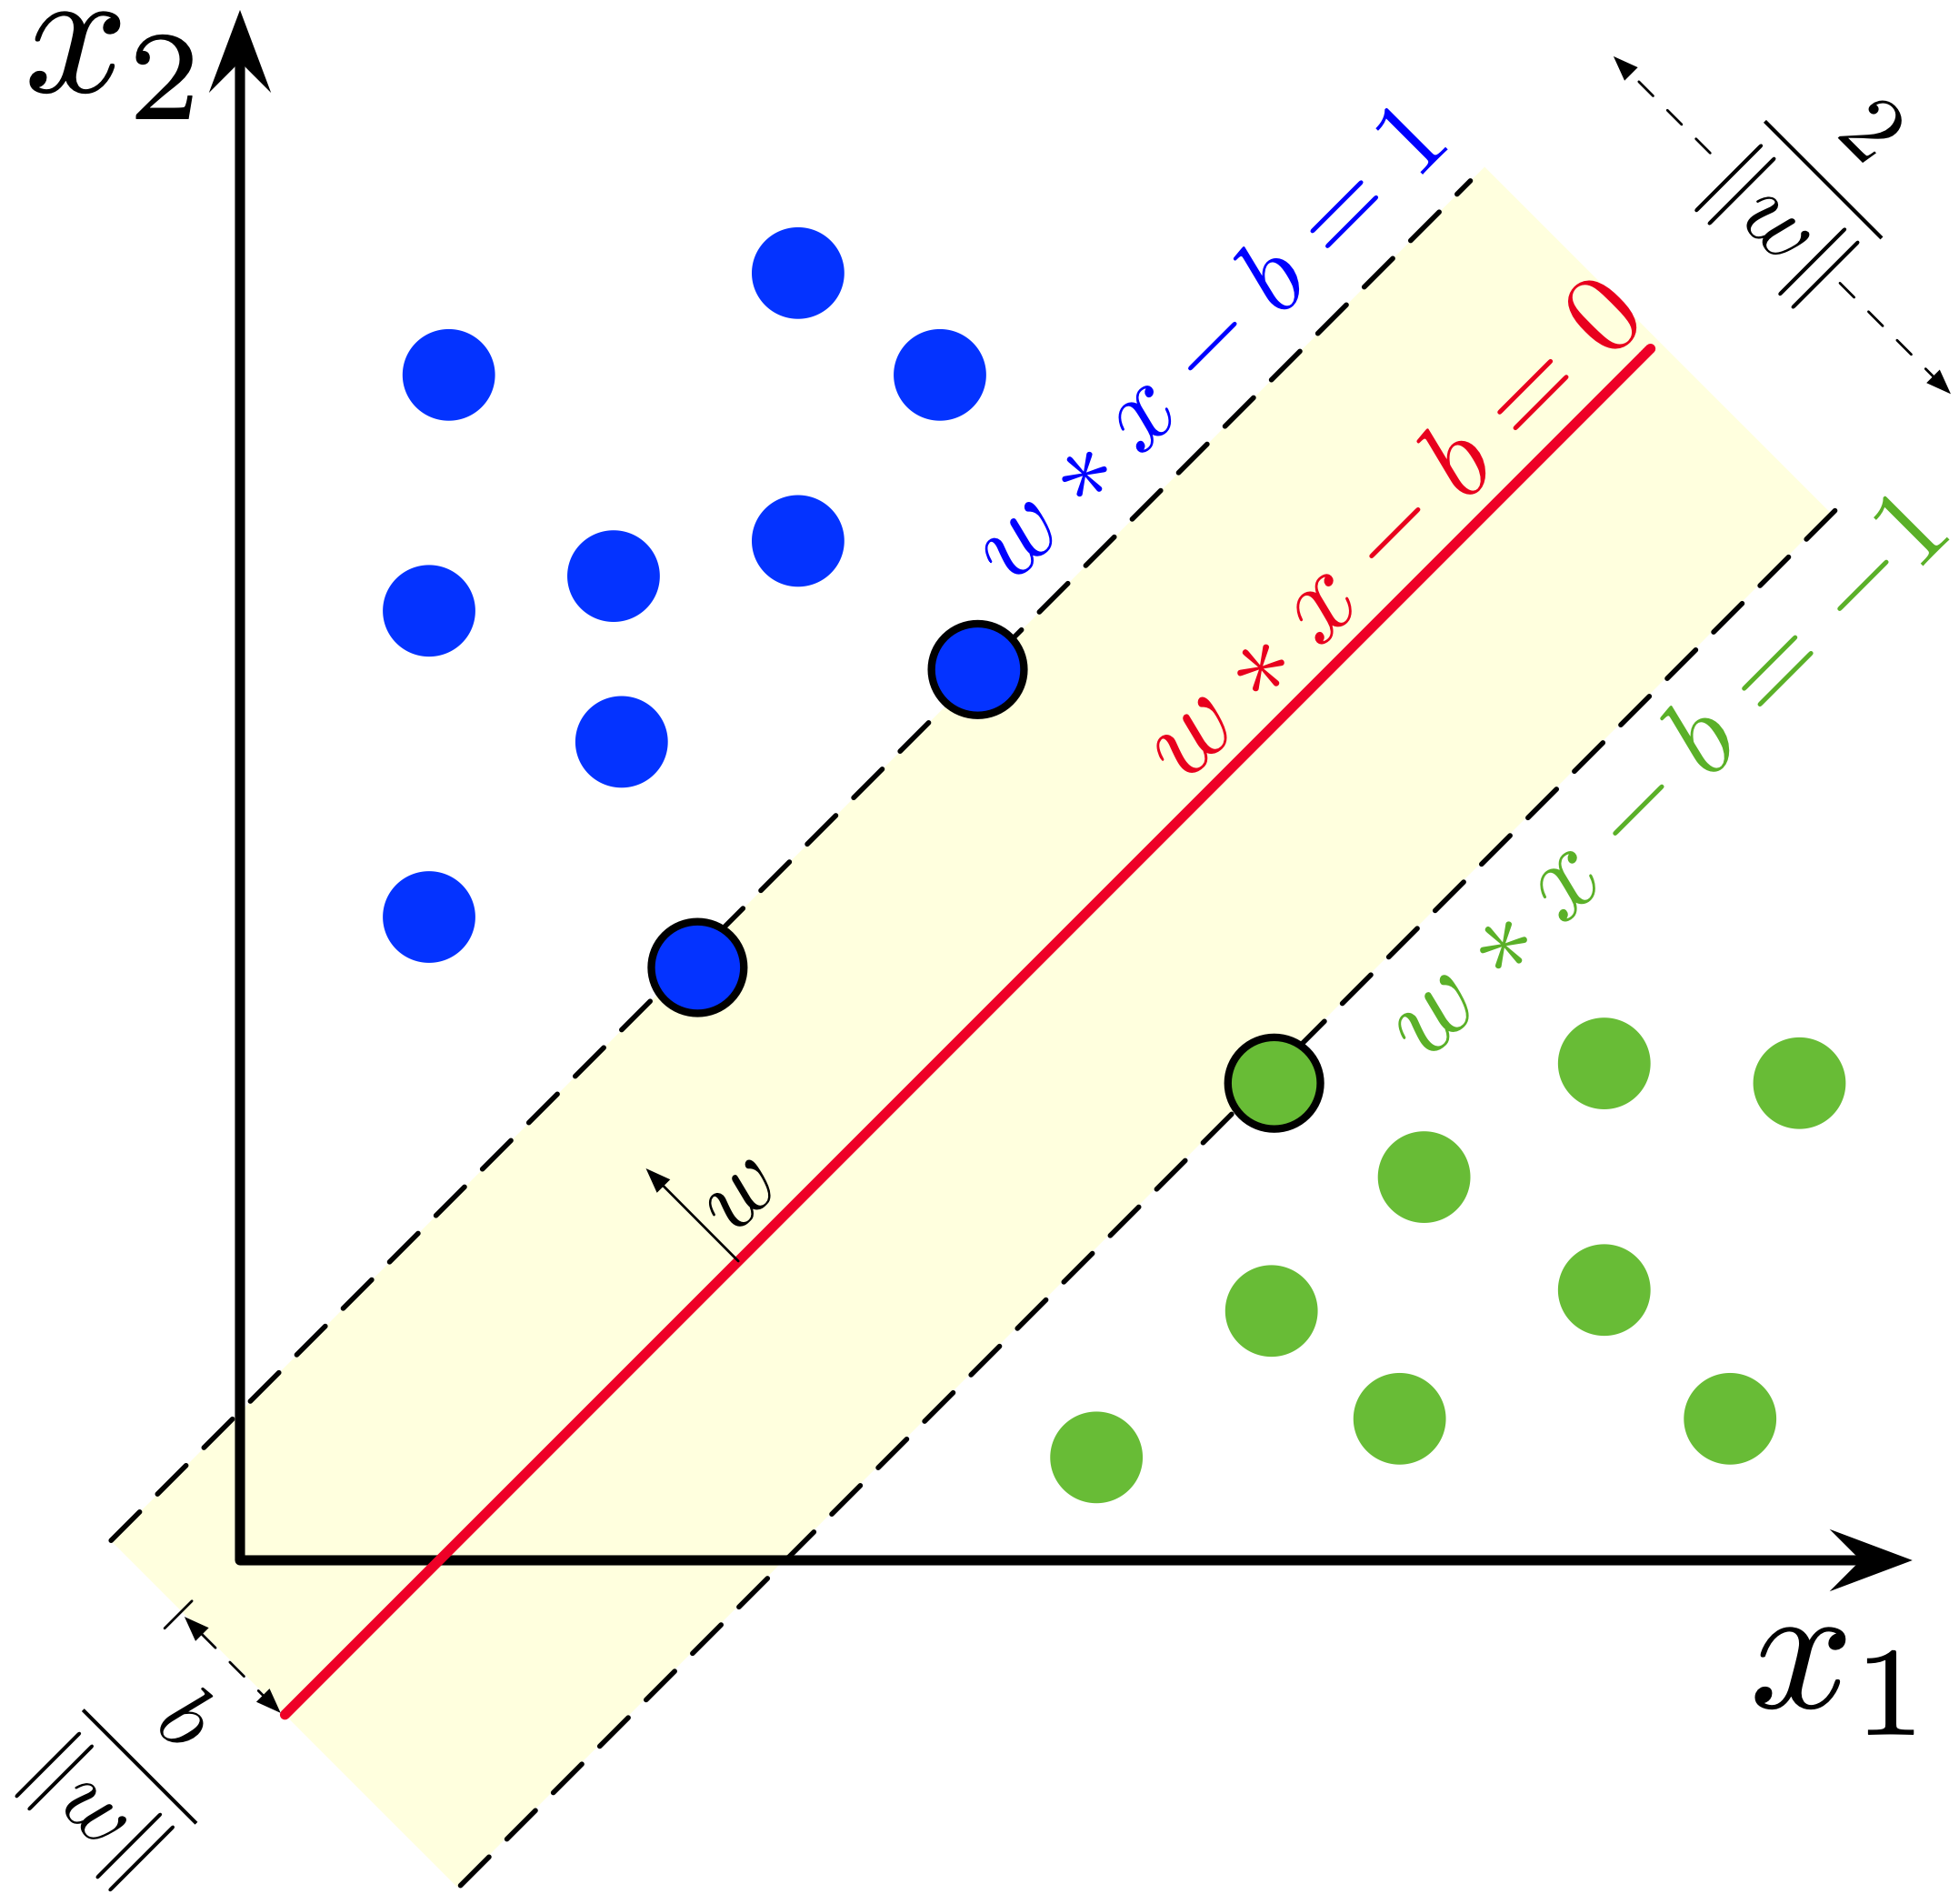
\includegraphics[width=0.9\textwidth]{images/SVM_margin.png}
        \label{fig:svm_margin}
    \end{figure}
    \end{column}
    
\begin{column}{0.6\textwidth}
\textit{Hard Margin Linear SVM}
\begin{itemize}
    \item Datos: $\{ \vec{x}_i,y_i\}$
    \item Clase objetivo: $y_i \in \{+1, -1\}$
    \item Ecuaci\'on del hiperplano
    $\vec{\omega} \cdot \vec{x} - b = 0$
    \item Restricciones: $y_i \vec{\omega} \cdot \vec{x} - b \geq 1$
    \item Se intenta minimizar $\|\omega\|$
    \item Se clasifica con la regla: $$sgn(\vec{\omega} \cdot \vec{x} - b)$$
\end{itemize}
\end{column}
\end{columns}    
\end{frame}
%-------------------------------------------------------------------------------
\begin{frame}{Support Vector Machines}
Para el caso no lineal se puede utilizar \textit{kernel tricks}.

Esto es reemplazar el producto escalar por un producto diferente por ejemplo:
\begin{itemize}
    \item $K(\vec{x}, \vec{y}) = (\vec{x} \cdot \vec{y})^d$
    \item $K(\vec{x}, \vec{y}) = exp(-\gamma \|\vec{x} - \vec{y}\|^2)$, $\gamma>0$
\end{itemize}
\begin{figure}
    \centering
    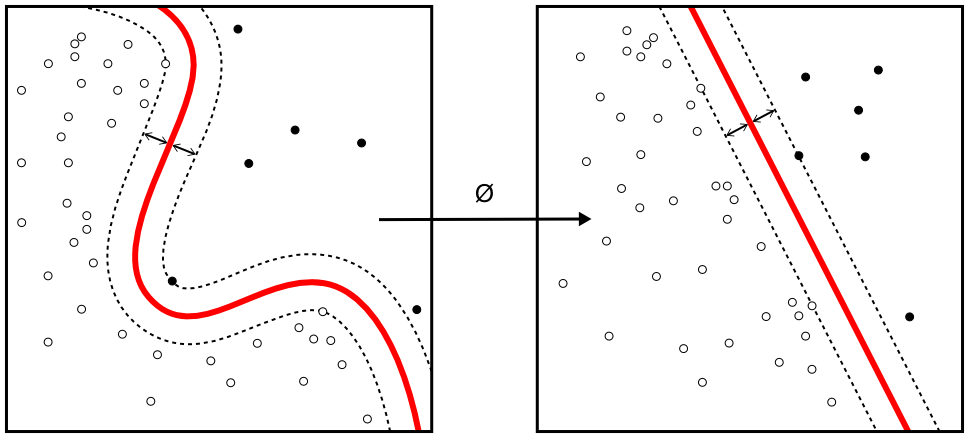
\includegraphics[width=0.3\textwidth]{images/Kernel_MachineSVM.png}
\end{figure}
\end{frame}
%-------------------------------------------------------------------------------
\begin{frame}{\'Arboles de Decisi\'on}
    \begin{columns}
    \begin{column}{0.5\textwidth}
    Estructura de \textit{dendograma}.
    Representaci\'on basada en reglas.
    
    Cada divisi\'on se determina maximizando el orden en el conjunto de datos.
    Metricas usadas para esto pueden ser \textit{Information Gain}, o impuridad de Gini.
    \end{column}
    
    \begin{column}{0.5\textwidth}
    \begin{center}
    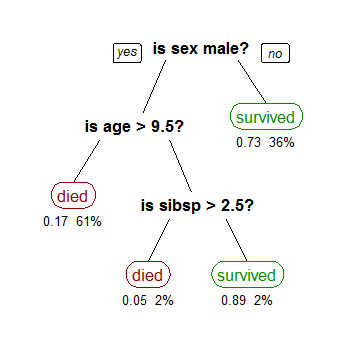
\includegraphics[width=0.45\textwidth]{images/CART_tree_titanic_survivors.png}
    \end{center}
    \end{column}
    
    \end{columns}
\end{frame}
%-------------------------------------------------------------------------------
\begin{frame}{Random Forest}
    
\end{frame}
%-------------------------------------------------------------------------------
\begin{frame}{Naive Bayes}
    Naive Bayes: utiliza el teorema de bayes para estimar probabilidades
    $$P(c=c_i|\vec{f}) = \frac{P(\vec{f}|c=c_i)P(c=c_i)}{P(\vec{f})}$$
\end{frame}
%-------------------------------------------------------------------------------
\begin{frame}{Perceptron}
    
\end{frame}
%-------------------------------------------------------------------------------
\begin{frame}{Evaluaci\'on: Tipos de errores}
Los errores en ML se extraen de la llamada \textbf{Matriz de Confusi\'on}, 
que representan los posibles escenarios de una prueba por Hip\'otesis:
\only<1>{
\small
\begin{center}
\begin{tabular}{|c|c|l|}
\hline
- & \multicolumn{2}{c|}{Decisi\'on}\\
\hline \hline
Condici\'on Real & Mantener $H_0$ & \multicolumn{1}{c|}{Rechazar $H_0$}\\
\hline
$H_0$ Verdadera & Acierto & \multicolumn{1}{c|}{Error de Tipo I}\\
\hline
$H_0$ Falsa & Error de Tipo II & \multicolumn{1}{c|}{Acierto}\\
\hline
\end{tabular}
\end{center}
}

\only<2>{
\small
\begin{center}
\begin{tabular}{|c|c|l|}
\hline
- & \multicolumn{2}{c|}{Decisi\'on}\\
\hline \hline
Condici\'on Real & Real & \multicolumn{1}{c|}{Falso}\\
\hline
Real & True Positive & \multicolumn{1}{c|}{False Negative}\\
\hline
Falso & False Positive & \multicolumn{1}{c|}{True Negative}\\
\hline
\end{tabular}
\end{center}
}

\end{frame}
%-------------------------------------------------------------------------------
\begin{frame} \frametitle{M\'etricas}
 %Los estad\'{i}sticos que miden el rendimiento de un test de decisi\'on son FDR, TPR, y FPR.
 \small
\begin{itemize}[<+->]
 \item \textbf{TPR} (o \textit{Tasa de Positivos Verdaderos}). Tambien es denominado \textbf{Recall}, simboliza la tasa de eventos seleccionados que realmente son positivos.
\item \textbf{FPR} (o \textit{Tasa de Falsos Positivos}) el cual es la probabilidad de cometer un \textbf{Error de Tipo II}, y representa la tasa de eventos seleccionados que no eran positivos.
\item \textbf{Precision} la tasa de eventos positivos dentro de los seleccionados como positivos.
\item \textbf{F1} es el promedio arm\'onico de las m\'etricas de Precisi\'on y Recall
$$F1 = (2 \times P \times R)/(P + R) $$
\end{itemize}
\end{frame}
%-------------------------------------------------------------------------------
\begin{frame} \frametitle{Figuras de M\'erito}
 \small
 \begin{columns}[T]
 \begin{column}{0.7\textwidth}
 \begin{figure}
 \centering
 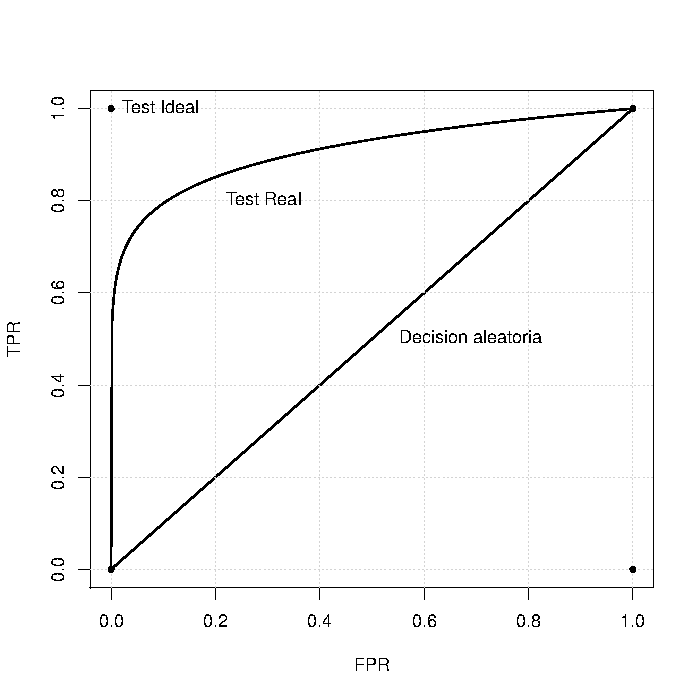
\includegraphics[width=0.85\textwidth]{./images/imgs_seminario1/ROC.png}
 % ROC.ps: 504x504 pixel, 72dpi, 17.78x17.78 cm, bb=0 0 504 504
 \caption{\scriptsize{Curva ROC}}
 %\label{fig:roc}
\end{figure}
\end{column}
\begin{column}{0.28\textwidth}
 Las tasas de FPR y TPR poseen un balance que se 
 caracteriza por la \textit{Respuesta Caracter\'{i}stica del Operador}.
% 
 AUC (\textit{\'Area Bajo la Curva} es una m\'etrica global.
%
 TPR y FPR, y sus derivadas \textit{son dados un valor umbral.})
 \end{column}
 \end{columns}
\end{frame}
%-------------------------------------------------------------------------------
\begin{frame}{Optimizaci\'on}

La optimizaci\'on es una rama totalmente independiente del ML.

Consiste en resolver problemas del siguiente tipo:
$$\vec{p} =  \argmax_x f(x) &= \{x \mid f(x) = \max_{x'} f(x')\}$$

Donde $f$ es la funci\'on evaluci\'on que queremos maximizar.
$\vec{p}$ ser\'an los par\'ametros elegidos finalmente para obtener el modelo entrenado.
\pause
Algunas de las m\'as utilizadas son:
\begin{itemize}
    \item Descenso por gradiente
    \item Cadenas de Markov
    \item B\'usqueda \textit{greedy}
    \item Algoritmos de tipo gen\'etico
\end{itemize}
\end{frame}
%-------------------------------------------------------------------------------
\section{Problemas del ML}
\begin{frame}{\textit{Overfitting}}
    \begin{itemize}
        \item El \textit{overfitting} o sobre-entrenamiento es el problema m\'as frecuente en ML.
        \item El fin ultimo de un algoritmo es la \textbf{generalizaci\'on}. Por esto aprender no es memorizar.
        \item Corresponde a la componente de la varianza del error.
    \end{itemize}
\end{frame}
%-------------------------------------------------------------------------------
\begin{frame}{\textit{Bias-Variance}}
\begin{columns}[T]
 \begin{column}{0.4\textwidth}
\begin{figure}
    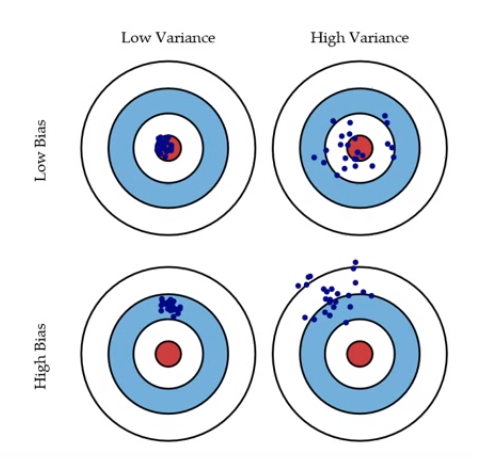
\includegraphics[width=\textwidth]{images/bias-variance.png}
    \label{fig:my_label}
\end{figure}
 \end{column}
\begin{column}{0.6\textwidth}
\\
El error en modelos predictivos ($M$) puede descomponerse en sesgo (bias) y varianza:
\begin{displaymath}
E\left[y_i-M(x_i)\right] = (Bias\left[M(x_i)\right])^2 + Var\left[M(x_i)\right]
\end{displaymath}
Existe un intercambio entre ambos, ya que ambos representan caras de la misma moneda: \textit{overfitting}
\end{column}
\end{columns}
\end{frame}
%-------------------------------------------------------------------------------
\begin{frame}{Validacion cruzada}
    
\end{frame}
%-------------------------------------------------------------------------------
\begin{frame}{\textit{k-Fold CV}}
    
\end{frame}
%-------------------------------------------------------------------------------
\section{El \textit{Deep Learning}}
\begin{frame}{Redes Neuronales Profundas}
    
\end{frame}
%-------------------------------------------------------------------------------
\begin{frame}{Redes Neuronales Convolucionales}
    
\end{frame}
%-------------------------------------------------------------------------------
\section{Aplicaciones en astronom\'ia}
%-------------------------------------------------------------------------------
\begin{frame}{Real/Bogus}
    
\end{frame}
%-------------------------------------------------------------------------------
% \begin{frame}{Open Source Fonts}
%  \begin{fullpageitemize}
%   \item {\montserratfont This is Montserrat}
%   \item {\notosansfont This is Noto Sans}
%   \item {\latolightfont This is Lato (light)}
%   \item {\inconsolatafont This is inconsolata}
%   \item \textsc{This is Alegreya Sans small caps}
%  \end{fullpageitemize}
% \end{frame}

% \begin{frame}{Color Palette}
%  \begin{center}
%   \crule[colordgray] \crule[colorhgray] \crule[colorblue] \crule[colorgreen] \crule[colororange]
%  \end{center}
% \end{frame}

% \framecard[colorgreen]{{\color{white}\hugetext{BIG BOLD TEXT}}}

% \framepic[0.8]{images/skeleton}{
%  \begin{textblock}{7}(7,2.5)
%     {\color{colorblue}\hugetext{\textbf{RUN!}}}
%  \end{textblock}
% }


\begin{frame}[allowframebreaks]
        \frametitle{Referencias}
        \tiny
        \bibliographystyle{apalike}
        \bibliography{bibliography.bib}
\end{frame}
\end{document}